\chapter{Исследовательский раздел}

В данном разделе приведен анализ характеристик разработанного ПО.

\section{Технические характеристики}

Технические характеристики устройства, на котором выполнялось тестирование и исследование, приведены ниже.

\begin{itemize}
	\item Операционная система: Ubuntu Linux 64-bit.
	\item Оперативная память: 16 GB.
	\item Количество логических ядер - 8.
	\item Процессор: Intel(R) Core(TM) i7-8850H CPU @ 2.60GHz \cite{intel}.
\end{itemize}

Тестирование проводилось на компьютере, включенном в сеть электропитания. Во время тестирования компьютер был нагружен только встроенными приложениями окружения рабочего стола, окружением рабочего стола, а также непосредственно системой тестирования. Во время тестирования оптимизации компилятора были отключены.

\section{Анализ алгоритмов по количеству сравнений}

На рисунках \ref{fig:lin_sc}, \ref{fig:bin_sc} и \ref{fig:seg_sc} приведены графики линейного, бинарного поиска и поиска по сегментам по количеству сравнений. В таблице 4.1 приведено соотвестсвие индексов названиям фильмов.

\begin{figure}[H]
	\centering
	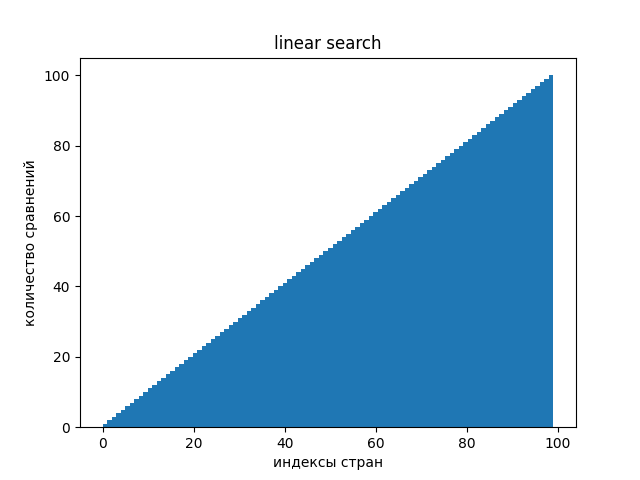
\includegraphics[scale=0.9]{inc/lin.png}
	\caption{График алгоритма линейного поиска.}
	\label{fig:lin_sc}
\end{figure}

По рисунку \ref{fig:lin_sc} можно сделать вывод, что сложность алгоритма линейного поиска зависит от индекса в словаре линейно.

\begin{figure}[H]
	\centering
	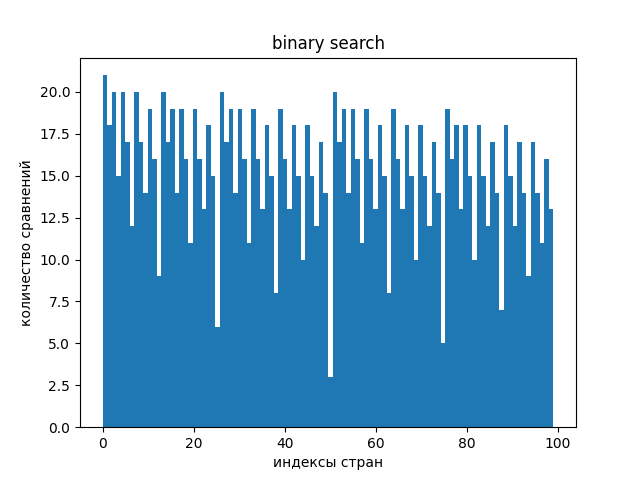
\includegraphics[scale=0.7]{inc/bin.png}
	\caption{График алгоритма бинарного поиска.}
	\label{fig:bin_sc}
\end{figure}

Можно заметить, что алгоритму бинарного требуется наименьшее число сравнений, когда элемент находится по центру массива. Из рисунков \ref{fig:lin_sc} и \ref{fig:bin_sc} следует, что худшему случаю бинарного поиска требуется в пять раз меньше сравнений, чем алгоритму линейного поиска.

\begin{figure}[H]
	\centering
	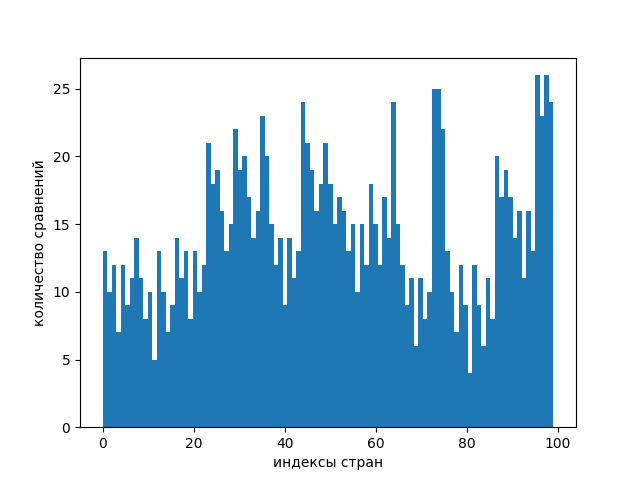
\includegraphics[scale=0.7]{inc/seg.png}
	\caption{График алгоритма поиска по сегментам.}
	\label{fig:seg_sc}
\end{figure}

В это случае число сравнений складывается из числа сравнений при линейном поиске сегмента и бинарном поиске в нем. На рисунке \ref{fig:seg_sc} видно, что нет прямой связи между индексом записи в исходном словаре и числе сравнений при поиске по сегментам.


На рисунках \ref{fig:lin_sc_sorted}, \ref{fig:bin_sc_sorted} и \ref{fig:seg_sc_sorted} приведена та же информация, отсортированная по количеству сравнений.

\begin{figure}[H]
	\centering
	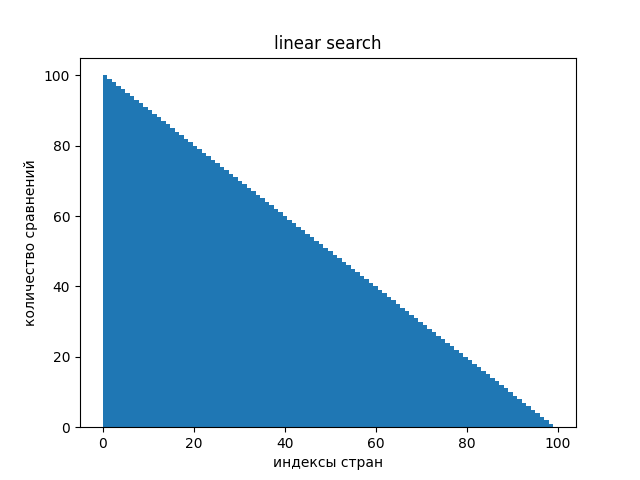
\includegraphics[scale=0.7]{inc/lin_sorted.png}
	\caption{График алгоритма линейного поиска.}
	\label{fig:lin_sc_sorted}
\end{figure}

\begin{figure}[H]
	\centering
	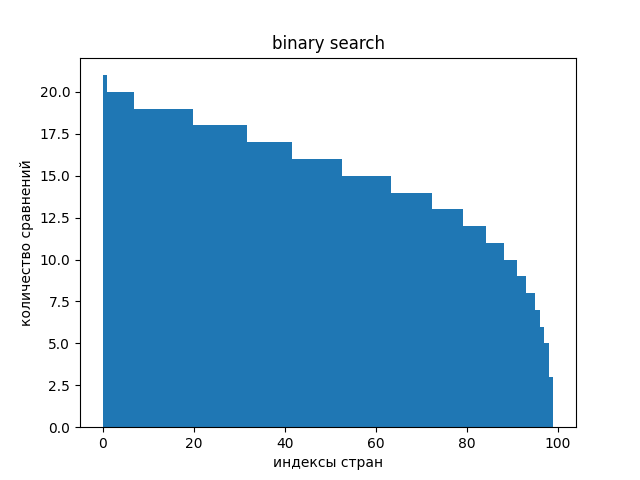
\includegraphics[scale=0.7]{inc/bin_sorted.png}
	\caption{График алгоритма бинарного поиска.}
	\label{fig:bin_sc_sorted}
\end{figure}

\begin{figure}[H]
	\centering
	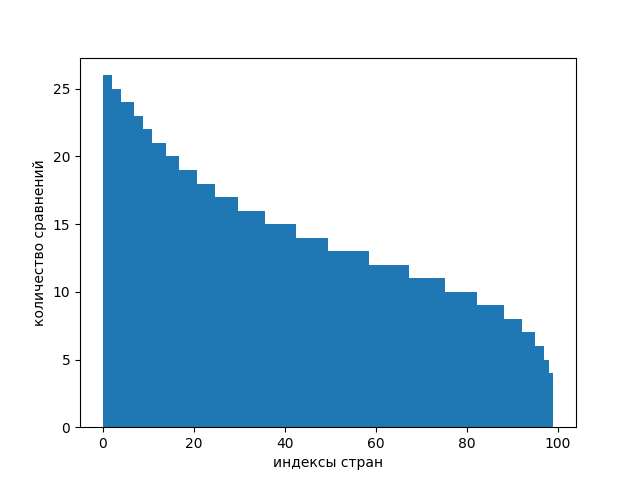
\includegraphics[scale=0.9]{inc/seg_sorted.png}
	\caption{График алгоритма поиска по сегментам.}
	\label{fig:seg_sc_sorted}
\end{figure}

\section{Вывод}

Исходя из полученных данных, можно сделать вывод, что алгоритм поиска в словаре, использующий частотный анализ, является боле эффективным, чем алгоритм полного перебора лишь в ряде случаев, в остальных же, он является менее эффективным, в связи с использованием сегментации и бинарным поиском внутри сегмента.

Отдельно отметим, что алгоритм бинарного поиска требует, в целом, меньшего числа сравнений, в связи с чем является более эффективным, чем алгоритм с частотным анализом. Однако, алгоритм бинарного поиска требует сортировки всего входного массива, что, в среднем случаи имеет сложность $O(nlog(n))$, в связи с чем алгоритм бинарного поиска становится менее эффективным, чем алгоритм частотного анализа, сортирующий данные по сегментам.

